\section{Ergebnisse}\label{sec:results}
% Fully corrected!
In den nachfolgenden Kapiteln werden die verschiedenen Resultate der Arbeit dargestellt und bereits die Leistung der KI in diversen Situationen abgebildet. Diese Untersuchung der Ergebnisse bietet eine wissenschaftliche Grundlage zur Identifikation der Schwachstellen der gewählten Modelle in der anschließenden Diskussion.

\subsection{Simulationsumgebung}
% Fully corrected!
Die erstellte Simulationsumgebung bietet abschließend die Möglichkeit Formel 1 Rennen auf Basis diverser Modelle zu generieren. Dabei wurden die Modelle durch Auswertung echter Renndaten erstellt und validiert. Die simulierten Rennen erlauben die Möglichkeit, die erforderliche Rundenzahl sowie die Anzahl der teilnehmenden Fahrzeuge frei zu wählen. Hierbei muss beachtet werden, dass die Referenzrundenzeit nicht einstellbar ist, da diese grundlegend in den diversen Modellen durch die Normierung der einzelnen untersuchten Stints auf die Referenzzeit von 80 Sekunden eingearbeitet wurde.
\\
Zusätzlich wurden umfassende Logging-Mechanismen zur Auswertung des aktuellen Verhaltens eines jeden Fahrzeuges in den Simulator integriert, um damit die Leistung des Simulators zu untersuchen, aber auch das Verhalten der KI in Relation zum restlichen Fahrerfeld untersuchen zu können.
\\
Zusammenfassend erfüllt der Simulator unsere Anforderungen und erlaubt somit das Training und die Validierung einer entsprechenden KI für Rennstrategie in der Formel 1. Grundlegend ist dabei die Entwicklung des Simulators aber nicht abgeschlossen, da jederzeit die angewandten Modelle hinterfragt und angepasst werden können und zudem die betrachteten Einflussfaktoren ausgeweitet werden könnten wie beispielsweise durch eine Untersuchung der Reifentemperatur.
\\\\
Die verschiedenen Modelle und deren Entwicklungshistorie werden im Folgenden dargestellt und erläutert. 

\subsubsection{Reifen Modelle}
% Fully corrected!
Die Reifen Modelle als zentraler Bestandteil unserer Simulation entstanden methodisch wie in \ref{sec:gen_models} beschrieben.\\
Die erste Iteration der gefundenen Modelle wies sich leider als fehlerhaft in der Methodik heraus und stellte keine realistische Abbildung des Reifenverhaltens dar. Diese Modelle wurden entsprechend nach der ersten Auswertung mit der KI als fehlerhaft erkannt. So repräsentierten diese Modelle einen einzelnen Fall eines Stints, zu sehen in Abbildung \ref{fig:tyre_model_single_stint} und nicht wie geplant die vollständige Auswertung über alle Stints, welche eine mindeste Anzahl an Runden beschrieben.
\begin{figure}[H]
    \centering
    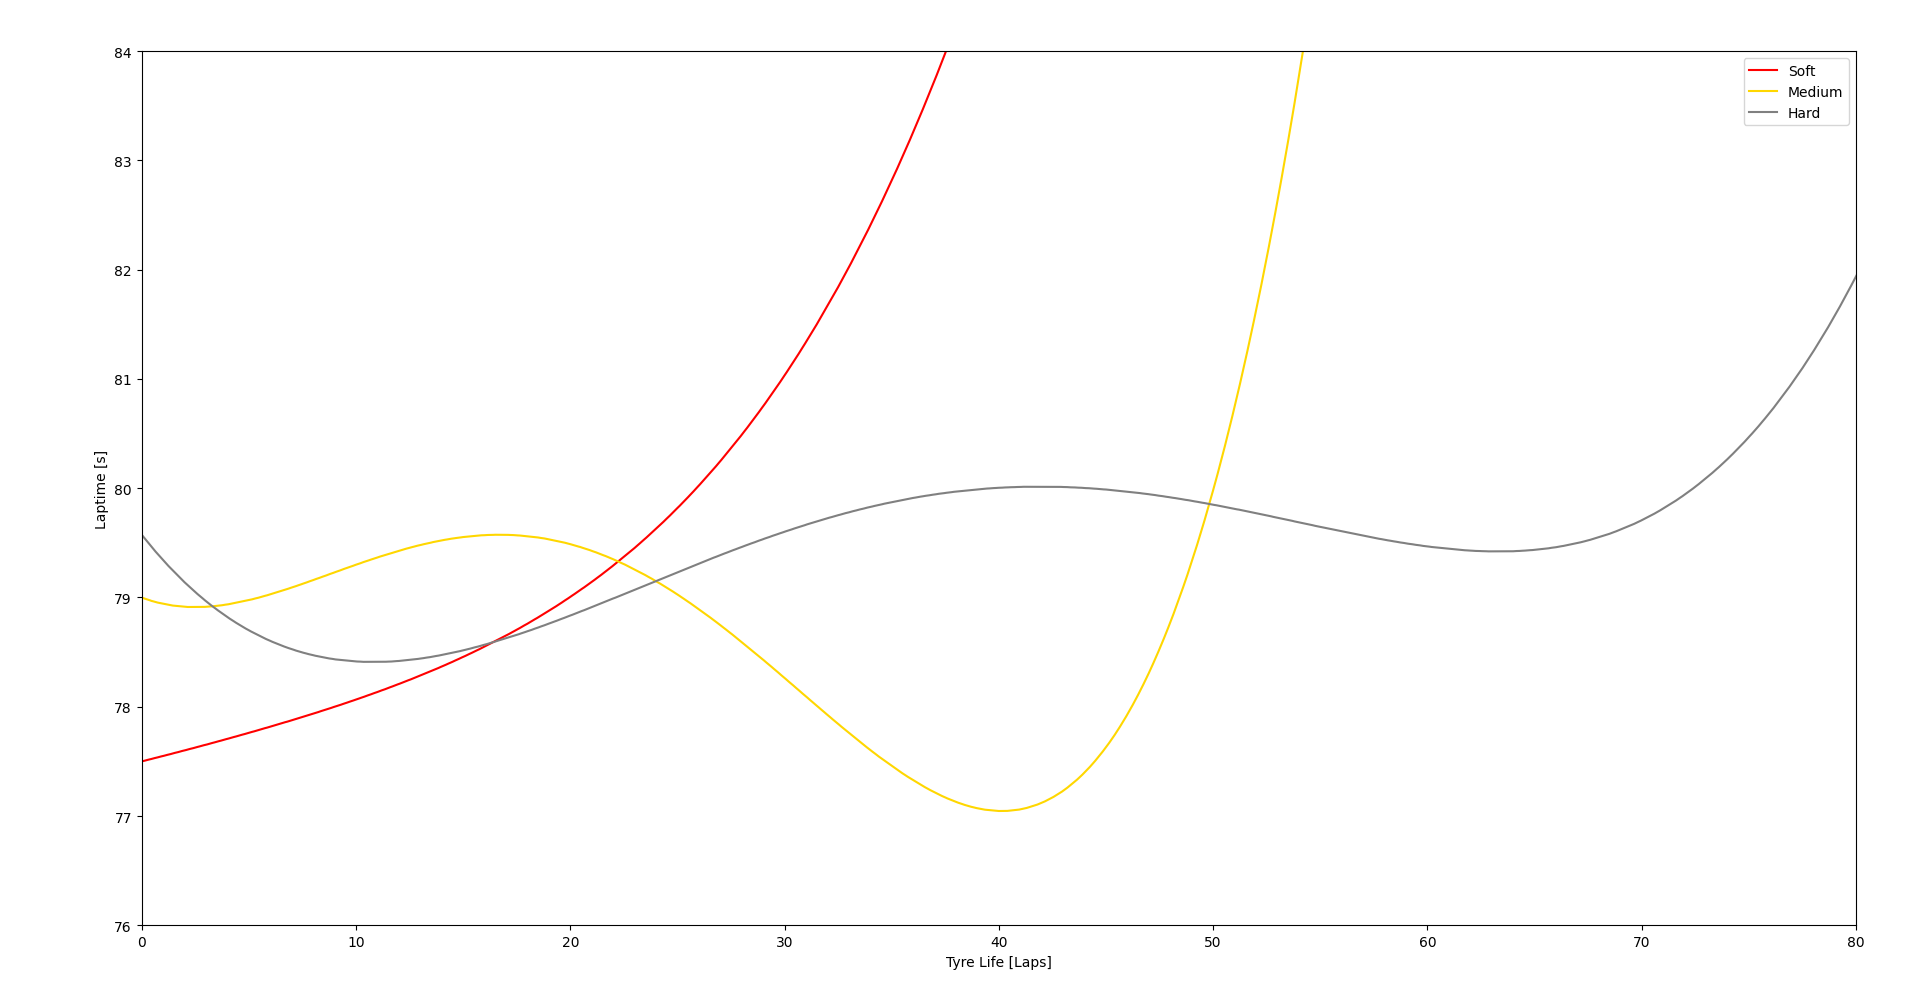
\includegraphics[scale=0.33]{Studienarbeit_F1/images/Tyre_models_better.png}
    \caption{Reifenverschleiß Modell über einen einzelnen Stint}
    \label{fig:tyre_model_single_stint}
\end{figure}
Dieses Modell ist entsprechend nicht repräsentativ und weißt sich besonders durch die starken Schwankungen über die Zeit des Stints aus. Diese sind einzelne Beobachtungen, welche nicht aussagekräftig für eine allgemeine Beschreibung des Reifens im Kontext eines allgemeinen Fahrzeuges sind. Dieses Modell ist im Kern problematisch aufgrund von sehr ausgeweiteten Stintlängen, welche beispielsweise den Soft mit einem Vorteil von bis zu zwei Sekunden pro Runde und einem kompetitiven Fenster von bis zu 35 Runden viel zu schnell abbilden .\\
Hierbei wurde in der Auswertung der Fehler gemacht, nur nach Stints zu filtern, welche mindestens eine gewisse Anzahl an Runden lang waren. Entsprechend wurden aber die statistischen Ausreißer nach oben weiterhin berücksichtigt und diese Einzelfälle, in welchen der Soft beispielsweise tatsächlich diese Leistungen erbracht hat, übermäßig berücksichtigt. Dies basierte auf der falschen Annahme, dass ein Stint umso länger dieser ist, repräsentativer für das Verhalten des Reifens wird. Grundlegend ist diese Annahme auch korrekt, da besonders kurze Stints wenig bis keine Aussage über den Verschleiß haben. Dennoch sollte für die Suche nach einem repräsentativen und realistischen Modell der Untersuchungsbereich nach oben hin limitiert sein, um nicht durch Ausreißer nach oben verfälscht zu werden. Dadurch werden Ausreißer in dieser Form nicht im Simulator auftreten können, was wiederum eine zusätzlich Abstraktion zur Wirklichkeit darstellt.
\\\\
Entsprechend dieser Beobachtung konnten die Auswertungen der einzelnen Reifenmodelle überarbeitet und korrektere Modelle aus dem Daten extrahiert werden. Diese Modelle, dargestellt in Abbildung \ref{fig:tyre_models_new}, beschreiben nun einen deutlich aussagekräftigeren Unterschied zwischen den einzelnen Reifentypen. Besonders gut zu sehen ist der lineare Verlauf des Verlusts an Gewicht in den Fahrzeugen, welches es erlaubt, über den Stint hinweg zunehmend schneller zu fahren, trotz des Verschleißes des Reifens. Mit Ende der Lebenszeit des Reifens, wie in \ref{sec:gen_models} beschrieben, greift aber dennoch der Verschleiß des Reifens und dieser baut zunehmend an Leistungspotential ab.\\
\begin{figure}
    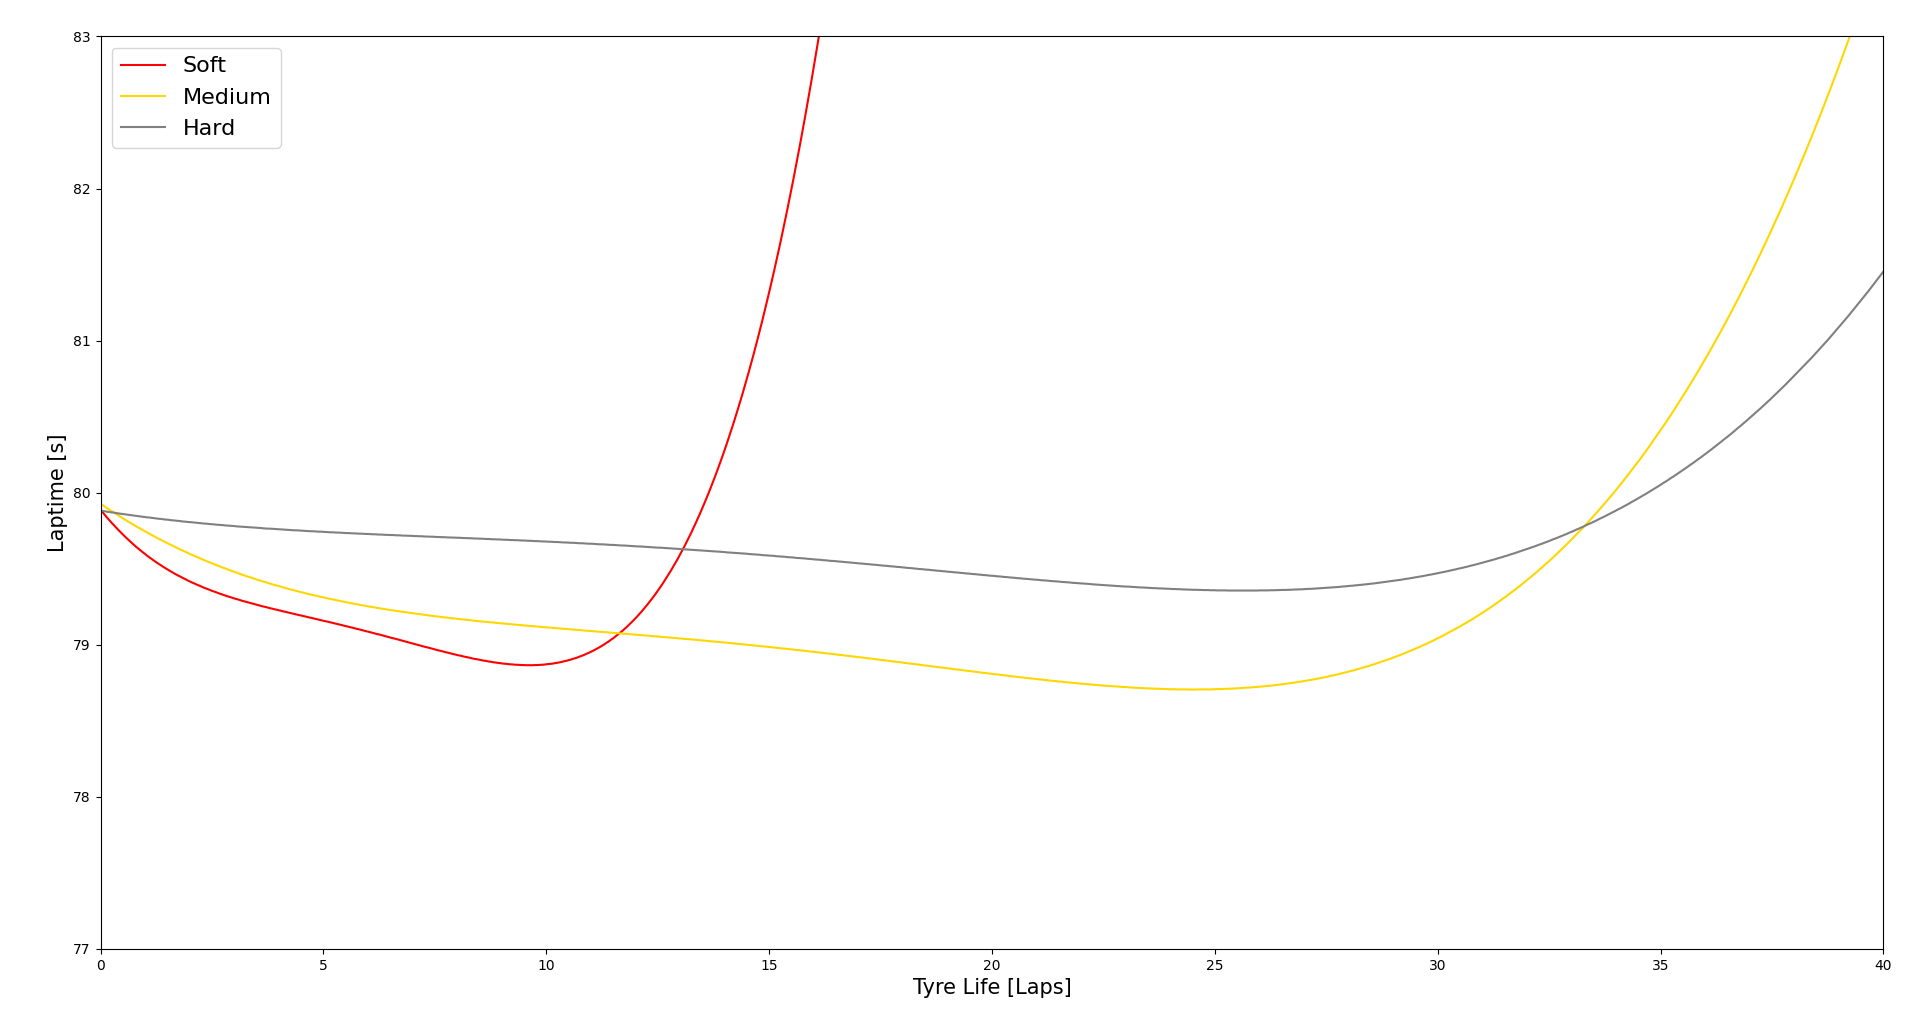
\includegraphics[scale=0.33]{Studienarbeit_F1/images/tyre_models_new_size.png}
    \caption{Abschließende Reifen Modelle}
    \label{fig:tyre_models_new}
\end{figure}

\subsubsection{Individuelles Leistungsmodell}
% Fully corrected!
Das individuelle Leistungsmodell soll, wie bereits in \ref{sec:gen_models}, den Leistungsparameter, welcher im Simulator durch einen Wert zwischen $[0,1]$ beschrieben ist, eines einzelnen Fahrzeuges in Kombination mit dem Fahrer auf den entsprechenden Zeitverlust pro Runde abbilden. Der Leistungsparameter des Fahrers ist ebenfalls im Intervall $[0,1]$ definiert. Entsprechend soll der beste Fahrer im besten Auto keine weitere Zeit auf seine Rundenzeit addiert bekommen, während der schlechteste Fahrer im schlechtesten Fahrzeug das maximale Zeitdelta erhält.\\
Aufgrund der Tatsache, dass die Leistung eines Fahrers direkt mit der Leistung des Fahrzeuges zusammenhängt, kann eine Auswertung und ein resultierendes Modell nicht mit einer solchen Genauigkeit die einzelnen Parameter direkt abbilden. Somit muss das gesuchte Modell die Leistung des Fahrzeuges und die Leistung des Fahrers kombiniert betrachten. Dadurch wird das gesuchte Modell im Intervall von $[0,2]$ die Zeitdifferenz pro Runde für ein Fahrzeug mit Fahrer abbilden.\\
Für diese Auswertung wurde die Saison 2021 betrachtet. Hierfür wurden die Zeiten der schlechtesten Kombination von Fahrer und Fahrzeug, was in diesem Fall dem russischen Piloten Nikita Mazepin des Teams \gqq{Haas F1} entspricht, mit der besten Kombination von Fahrer und Fahrzeug auf die mittlere Differenz der Rundenzeiten untersucht. Als optimal Fall wurde der britische Fahrer Lewis Hamilton im Mercedes betrachtet. Resultat dieser Auswertung ist das Modell in Abbildung \ref{fig:individual_model}.
\begin{figure}
    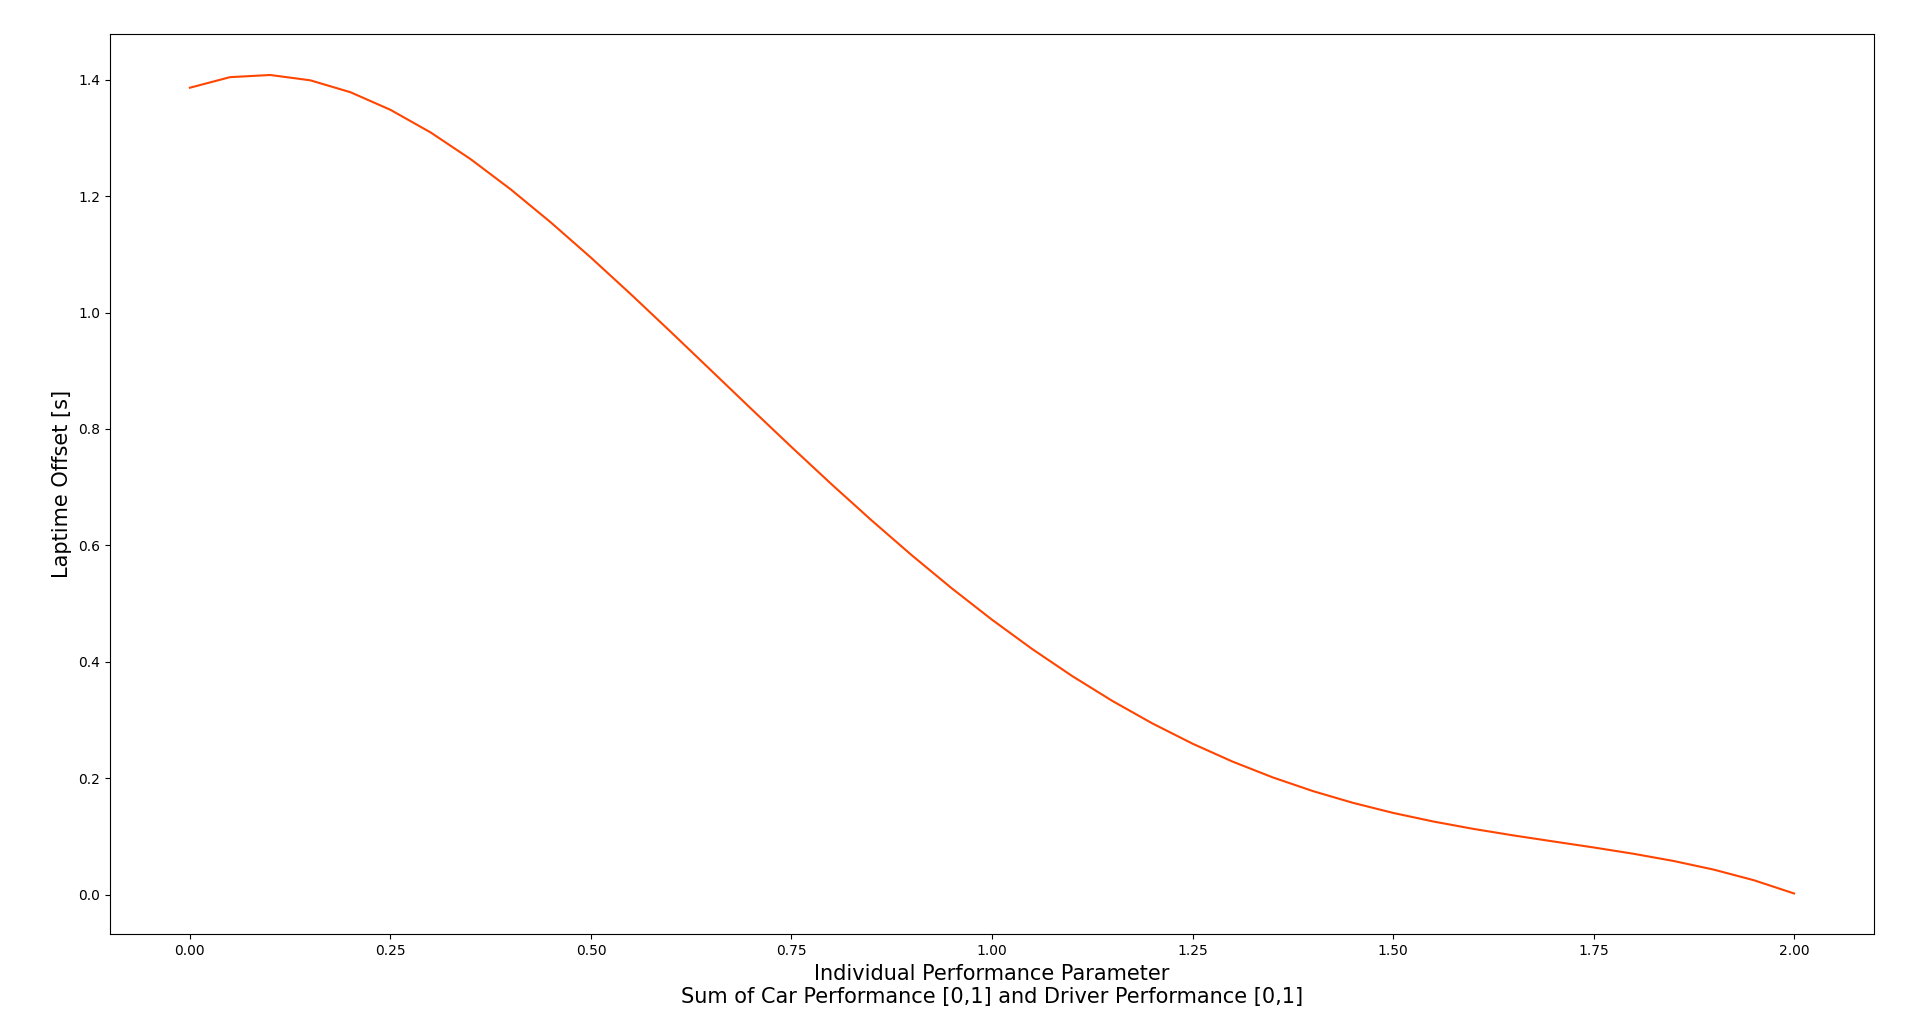
\includegraphics[scale=0.33]{Studienarbeit_F1/images/indivu_model_new_size.png}
    \caption{Individuelles Leistungsmodell}
    \label{fig:individual_model}
\end{figure}

Folgend dem Modell fährt ein Fahrzeug mit Leistungsparameter $0$ im Schnitt $1.4$ Sekunden langsamer pro Runde auf eine Rundenzeit von 80 Sekunden. Im mittleren Leistungsbereich, in welchem sich die meisten Fahrzeuge befinden, sind etwa eine zeitliche Differenz von $0.2$ - $0.5$ Sekunden pro Runde im Vergleich zum Optimum gegeben.

\subsubsection{Wechselwirkungsmodell}
% Fully corrected!
Das eingesetzte Wechselswirkungsmodell folgt dem Ziel, die in \ref{sec:race_behaviour} beschriebenen Einwirkungen von anderen Fahrzeugen auf ein einzelnes Fahrzeug abzubilden. Demnach muss das Modell den zusätzlichen Reifenverschleiß beim dichten Folgen eines anderen Fahrzeuges abbilden können, um somit den Verlust an aerodynamischen Abtrieb zu simulieren. \\
Zusätzlich muss entschieden werden, wie ein Überholmanöver stattfinden kann, sodass die Reihenfolge im Simulator konsistent bleibt. Zusätzlich soll ein Überholmanöver leichter gelingen, sollte der \gqq{Angreifer} ein schnelleres Tempo fahren können. Es muss also entschieden werden, ab wann die Möglichkeit zum Überholen besteht und unter welchen Umständen das Überholmanöver das Potential zu gelingen hat. Dies geschieht unter Berücksichtigung der Verteidigung durch das vorausfahrende Fahrzeug.\\
\\
Grundlegend wird davon ausgegangen, dass erst bei einem zeitlichen Delta von unter einer Sekunde zwischen zwei Fahrzeugen die Betrachtung des gegenseitigen Einflusses betrachtet werden muss. Innerhalb dieses Fensters ist ein Überholmanöver möglich, da das Auftreten des Windschattens eine erhöhte Spitzengeschwindigkeit auf den Geraden erlaubt. Dieser Windschatten verursacht aber wiederum in den Kurven, dass die Reifen mehr strapaziert werden müssen, um die Geschwindigkeit aufgrund des fehlenden Abtriebs zu halten. Entsprechend wurde diese Grenze als Schwellwert für die Betrachtung beider Wechselwirkungsmodelle genutzt.\\\\
Sollte nun ein Fahrzeug unter einer Sekunde hinter dem vorausfahrenden Fahrzeug sein, so wird das Alter des Reifens pro Runde zusätzlich um einen Faktor zwischen $[0.05, 0.25]$ erhöht. Dieses Intervall wurde abhängig vom Abstand zum vorausfahrenden Fahrzeug gemacht, um somit die verstärkende Wirkung bei abnehmenden Abstand zu repräsentieren. Das generierte Modell ist in Abbildung \ref{fig:add_tyre_degradation} zu sehen.\\
\begin{figure}
    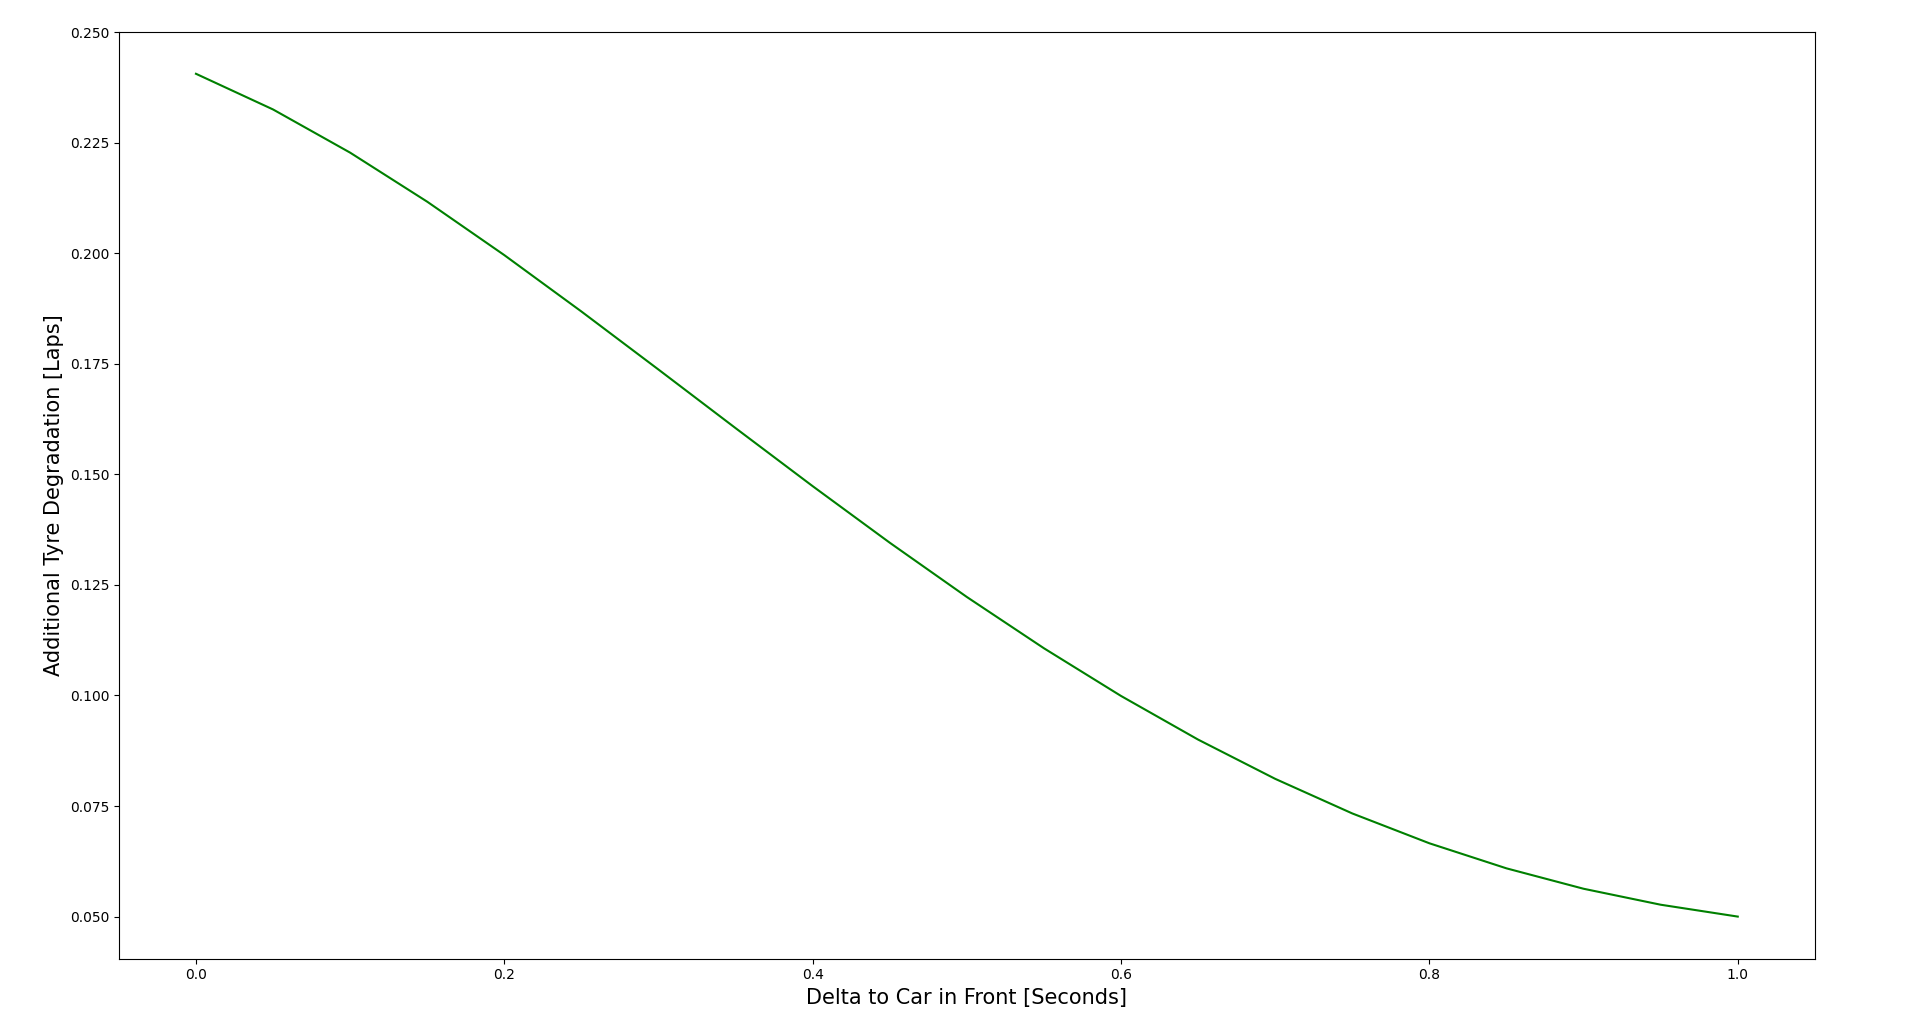
\includegraphics[scale=0.34]{Studienarbeit_F1/images/tyre_deg_new_size.png}
    \caption{Wechselwirkungsmodell für zusätzlichen Reifenverschleiß}
    \label{fig:add_tyre_degradation}
\end{figure}

\subsection{KI Modell}
% Tims Stuff :D
Als Basis für die finale KI zur Optimierung der Rennstrategie dienen die in Kapitel \ref{künstliche_Intelligenz} erarbeiteten Sachverhalte. Als RL-Algorithmus wurde sich aufgrund der Tests mit der einfachen KI für den \gqq{double-DQN} entschieden. Die zentrale Änderung des finalen Modells stellt die Größe des Zustands als Eingabe für das neuronale Netz dar. Dieser beinhaltet nun die gesamte verfügbare Information über denn Rennzustand. Eine Übersicht über die im Wesentlichen verfügbaren Informationen lässt sich in Abbildung \ref{fig:race_state} finden.
\begin{figure}
    \centering
    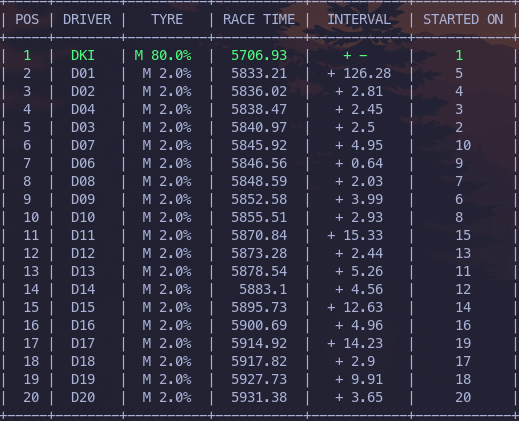
\includegraphics[scale=0.7]{Studienarbeit_F1/images/race_state.png}
    \caption{Verfügbare Informationen über jedes Auto am Ende eines Rennens}
    \label{fig:race_state}
\end{figure}
Zusätzlich wird für die Information über die bereits genutzten Reifentypen in Form eines Flags übergeben, um die Assoziation einer Disqualifikation mit der Nutzen von einer zu geringen Anzahl von verschiedenen Reifentypen zu ermöglichen. Eine vollständige Aufschlüsselung des Eingabezustands wie er im Code vorbereitet wird lässt sich in Listing \ref{lst:race_state} betrachten.

\begin{lstlisting}[label={lst:race_state}, caption={Ermittlung des Eingabezustands des neuronalen Netzes}, language={Python}]
def get_state(car: Car, lap : int):
    """
    return the current state for the AI - Input
    """
    # tyre degredation from 100% to 0%
    degredation = car.tyre.degredation * 100
    remaining_laps = RACE_DISTANCE - lap
    delta_to_leader = car.delta_to_leader
    # last lap time of the car
    lap_time = car.last_lap_time
    position = car.position
    # one hot coded : which compound is the car on?
    soft, medium, hard = one_hot_compound(car.tyre.compound)
    # have we used enough different compounds to not be disqualified?
    second_compound_flag = 1 if car.distinctUsedTyreTypes() >= 2 else 0
    delta_to_front = car.delta_to_car_infront if car.delta_to_car_infront != "-" else 0
    starting_pos = car.grid_position
    state_tensor = torch.tensor([degredation, remaining_laps, delta_to_leader, lap_time, position, soft, medium, hard, second_compound_flag, delta_to_front, starting_pos], dtype=torch.float32)

    return state_tensor
\end{lstlisting}
Basierend auf diesem Eingabezustand wurden die Hyperparameter des DQN manuell ermittelt. Einige der Parameter, die sich beim Ermittlungsprozess als besonders einflussreich herausgestellt haben, sind in Listing \ref{lst:hyperparams} dargestellt.
\begin{lstlisting}[label={lst:hyperparams}, caption={Ausgewählte, wichtige Hyperparameter des DQN}, language={Python}]
   layers = [11, 30, 30, 4]
   learning_rate = 1.5 * 1e-4
   episodes = 20000
   # keep 200 races in memory
   memory_size = 200 * race_length
   # amount of steps in the environment until memory is sampled
   sampling_period = 5
   # amount of transitions to sample from memory
   batchsize = 32
\end{lstlisting}

\subsection{KI Performance}\label{sec:ai_performance}
Abschließend gilt es die Leistung und das Verhalten eines trainierten Modells zu analysieren und zu vergleichen. Dabei können die von der KI erlernten Strategien untersucht und in Kontext der realen Verhältnisse gesetzt werden. Hierzu werden verschiedene Szenarien mit einem vortrainierten Modell untersucht, dabei soll insbesondere das Verhalten der KI in extremen Szenarien, welche als Grenzfälle betrachtet werden können, analysiert werden. Die Szenarien unterscheiden sich dabei einerseits in die Startposition des KI-Fahrzeuges sowie in der Leistung des Autos. Das untersuchte Modell sollte im Training jede Start-Position bereits erfahren haben und sollte sich dabei in verschieden starken Fahrzeugen befanden haben.\\\\
Bei der Betrachtung der Performance gilt es die Stabilität der Resultate der KI über eine Vielzahl von Rennen zu betrachten, um so zum einen eine Aussage über die Realitätsnähe des Simulators sowie die Leistungsfähigkeit und Qualität der KI machen zu können.\\
Das restliche Feld, mit welchem die KI konkurriert, fährt dabei eine statische Strategie. Diese Strategie ist durch vorangegangene Test gewählt, da diese statische Strategie oft von der KI gewählt und genutzt wurde. Somit startet das Feld auf Softs und fährt in den Runden 15 und 45 an die Box und wechselt dabei auf Mediums. 

\subsubsection{Szenario 1: Leistungsstärkstes Auto auf Pole-Position}\label{sec:best_car_pole}
Das nachfolgend betrachtete Szenario entspricht vor dem Hintergrund seiner Situationsparameter der optimalen Ausgangslage eines Teilnehmenden in der Formel 1.\\
Der Teilnehmende startet von der vordersten Start-Position und hat aus diesem Grund eine vorteilhafte Position innerhalb des Rennens inne. Außerdem hat das untersuchte Fahrzeug die stärksten Leistungsparameter mit den Werten für Fahrerleistung und für Fahrzeugleistung jeweils gleich eins.\\
Dieses Szenario erlaubt die Untersuchung, ob die KI tatsächlich eine optimale Strategie wählt und entsprechend die Start-Position beziehungsweise die Führung halten kann oder sogar den Abstand zum ersten Verfolger ausbauen kann. Diese Erwartung gegenüber des Szenarios wird durch den Umstand des performantesten Fahrzeuges zusätzlich verstärkt. Es ist somit zu erwarten, dass bei der Betrachtung einer Vielzahl von Renndurchläufen insgesamt die Anzahl der erreichten ersten Plätze in der Gesamtheit aller Rennsimulationen massiv überwiegen sollte.
\\
\begin{figure}
    \centering
    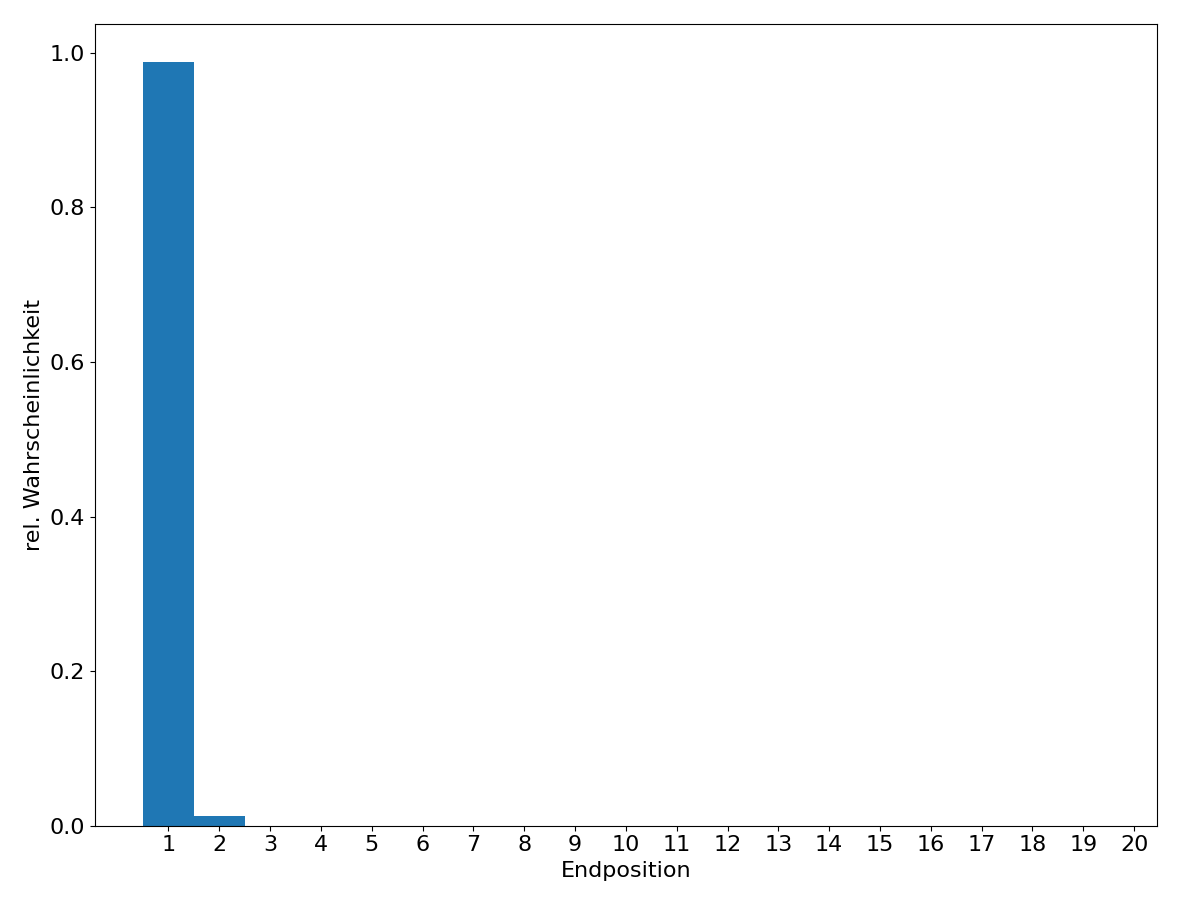
\includegraphics[scale=0.5]{Studienarbeit_F1/images/hist_best_car_pole.png}
    \caption{Szenario 1: Anteile der Platzierungen bei 1000 Renndurchläufen}
    \label{fig:hist_best_car_pole}
\end{figure}
\\
Zur Untersuchung der Stabilität und längerfristigen Performance der KI wurden die Rennergebnisse über 1000 Renndurchläufe bei den zuvor genannten Parametern betrachtet und ausgewertet. Die dabei erreichten Rennplatzierungen sind in Abbildung \ref{fig:hist_best_car_pole} in Form eines Histogramms dargestellt.\\
Hierbei zeigt sich bis auf einen sehr kleinen Anteil an zweiten Plätzen eine Bestätigung des erwarteten Verhaltens in Form eines großen relativen Anteils von Rennsiegen.\\
Dieses stabile Verhalten unterstreicht die Performance der KI. Es gelingt in der absoluten Mehrzahl der Fälle, die Führungsposition gegen die Konkurrierenden im Feld zu verteidigen. Der seltene Fall des zweiten Platzes kann als Bestätigung der Performance interpretiert werden, da maximal eine einzige Platzierung gegenüber den Konkurrierenden eingebüßt wird.
\\
\begin{figure}
    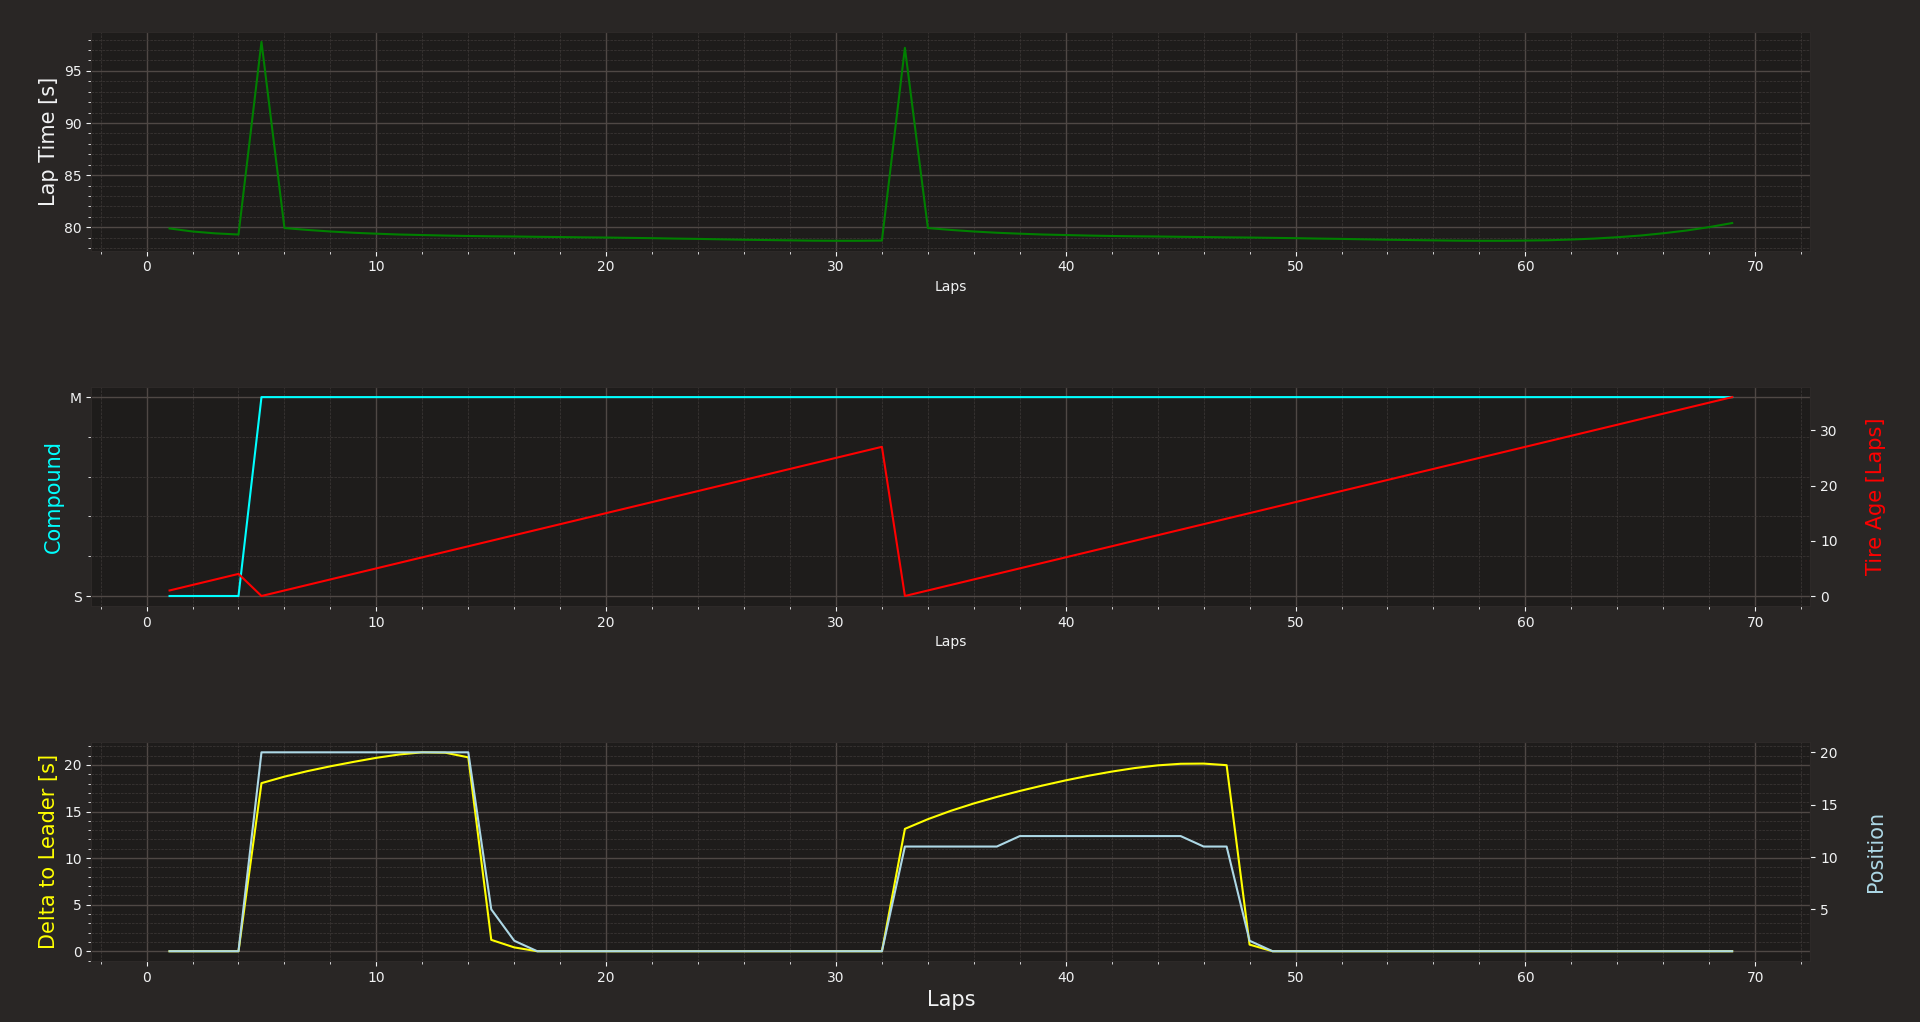
\includegraphics[scale=0.325]{Studienarbeit_F1/images/eval_best_pole_stayed_first.png}
    \caption{Beispielhaftes Verhalten Szenario 1 - Start von Pole - Platz 1 im Ziel}
    \label{fig:example_scenario_one}
\end{figure}
\\
Zur Veranschaulichung des Verhaltens der KI über ein einzelnes Rennen hinweg sind in Abbildung \ref{fig:example_scenario_one} die Abläufe eines einzelnen Rennens dargestellt. Im obersten Graph findet sich die Rundenzeit der KI wieder, Hier sind die zwei gewählten Boxenstopps der KI deutlich als Ausreißer nach oben zu erkennen. Hierbei startet die KI auf Soft und wechselt anschließend zwei Mal auf Mediums.\\
Entsprechend verliert die KI die Führung, welche sie aber mit dem Boxenstopp des restlichen Feldes wiedererlangen kann.\\
Aus analytischer Sicht zeigt der Rennsimulator sehr aussagekräftige und realistische Verhältnisse in diesem Szenario. So ist Überholen möglich und machbar, aber auch nicht zu einfach. Aus strategischer Sicht ist hierbei interessant, dass die KI beide Boxenstopps früher ansetzt als das restliche Feld und dadurch sogar kurzzeitig den letzten Platz belegt. Dieser frühere Boxenstopp aber offensichtlich der gesamten Rennzeit nicht schadet und die KI somit den Sieg halten kann trotz des zunehmenden Verschleißes am Ende des Rennens.

\subsubsection{Szenario 2: Leistungsschwächstes Auto auf Pole-Position}
% Car Parameters = 0.4
Das folgende Szenario soll ein Rennen von der Pole-Position aber dafür im Auto mit den schlechtesten Individual-Leistungswerten abbilden. Dies dient rein zur wissenschaftlichen Untersuchung des Verhaltens der KI und des Simulators, da das Szenario in der realen Formel 1 sehr unrealistisch ist. Entsprechend erlaubt diese Analyse besonders Rückschlüsse auf die Korrektheit der eingesetzten Modelle im Simulator.\\
Es wird also erwartet, dass das Fahrzeug auch bei durch die KI optimierter Strategie im Fahrerfeld stark zurückfallen wird und somit das Rennen außerhalb der Top 10 beenden sollte.\\
\begin{figure}
    \centering
    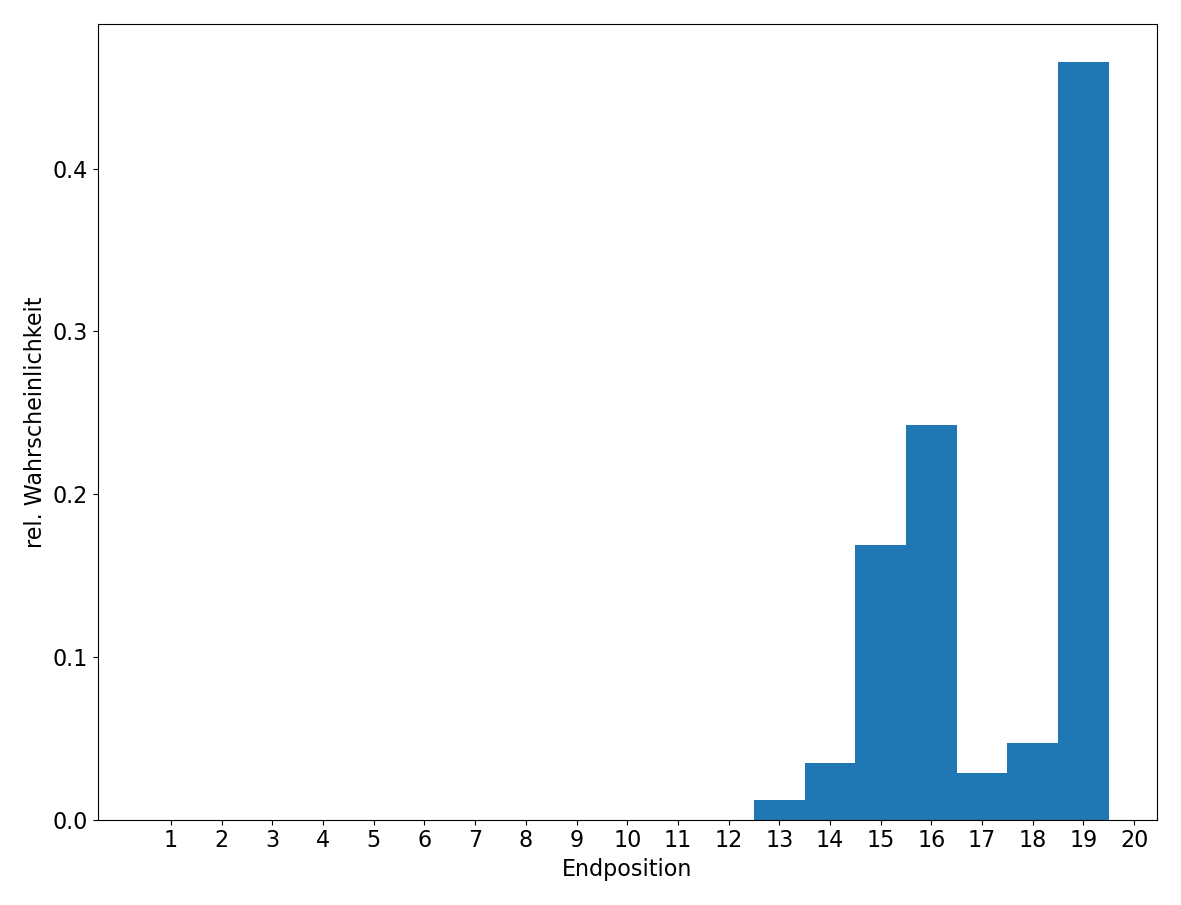
\includegraphics[scale=0.5]{Studienarbeit_F1/images/hist_worst_car_pole.png}
    \caption{Szenario 2: Anteile der Platzierungen bei 1000 Renndurchläufen}
    \label{fig:hist_worst_car_pole}
\end{figure}
Eine Betrachtung der Resultate über 1000 Rennen liefert auch in diesem Szenario eine Bestätigung der zuvor aufgestellten These hinsichtlich der erwarteten Leistungen der KI innerhalb des Rennens. In der Abbildung \ref{fig:hist_worst_car_pole} ist zu erkennen, dass trotz der zunächst optimalen Ausgangslage am Beginn des Rennens kein Ergebnis unter den Top 10 erzielt werden konnte, sondern sich die Resultate im letzten Drittel des Feldes konzentrieren. Diese Auswertung bestätigt den signifikanten Einfluss der Leistungsparameter auf die schlussendlichen Rennresultate. Es wird der Realität entsprechend aufgezeigt, dass trotz einer potenziell optimalen Rennstrategie in einem nicht konkurrenzfähigen Auto keine guten Platzierungen erreicht werden können.\\
\begin{figure}
    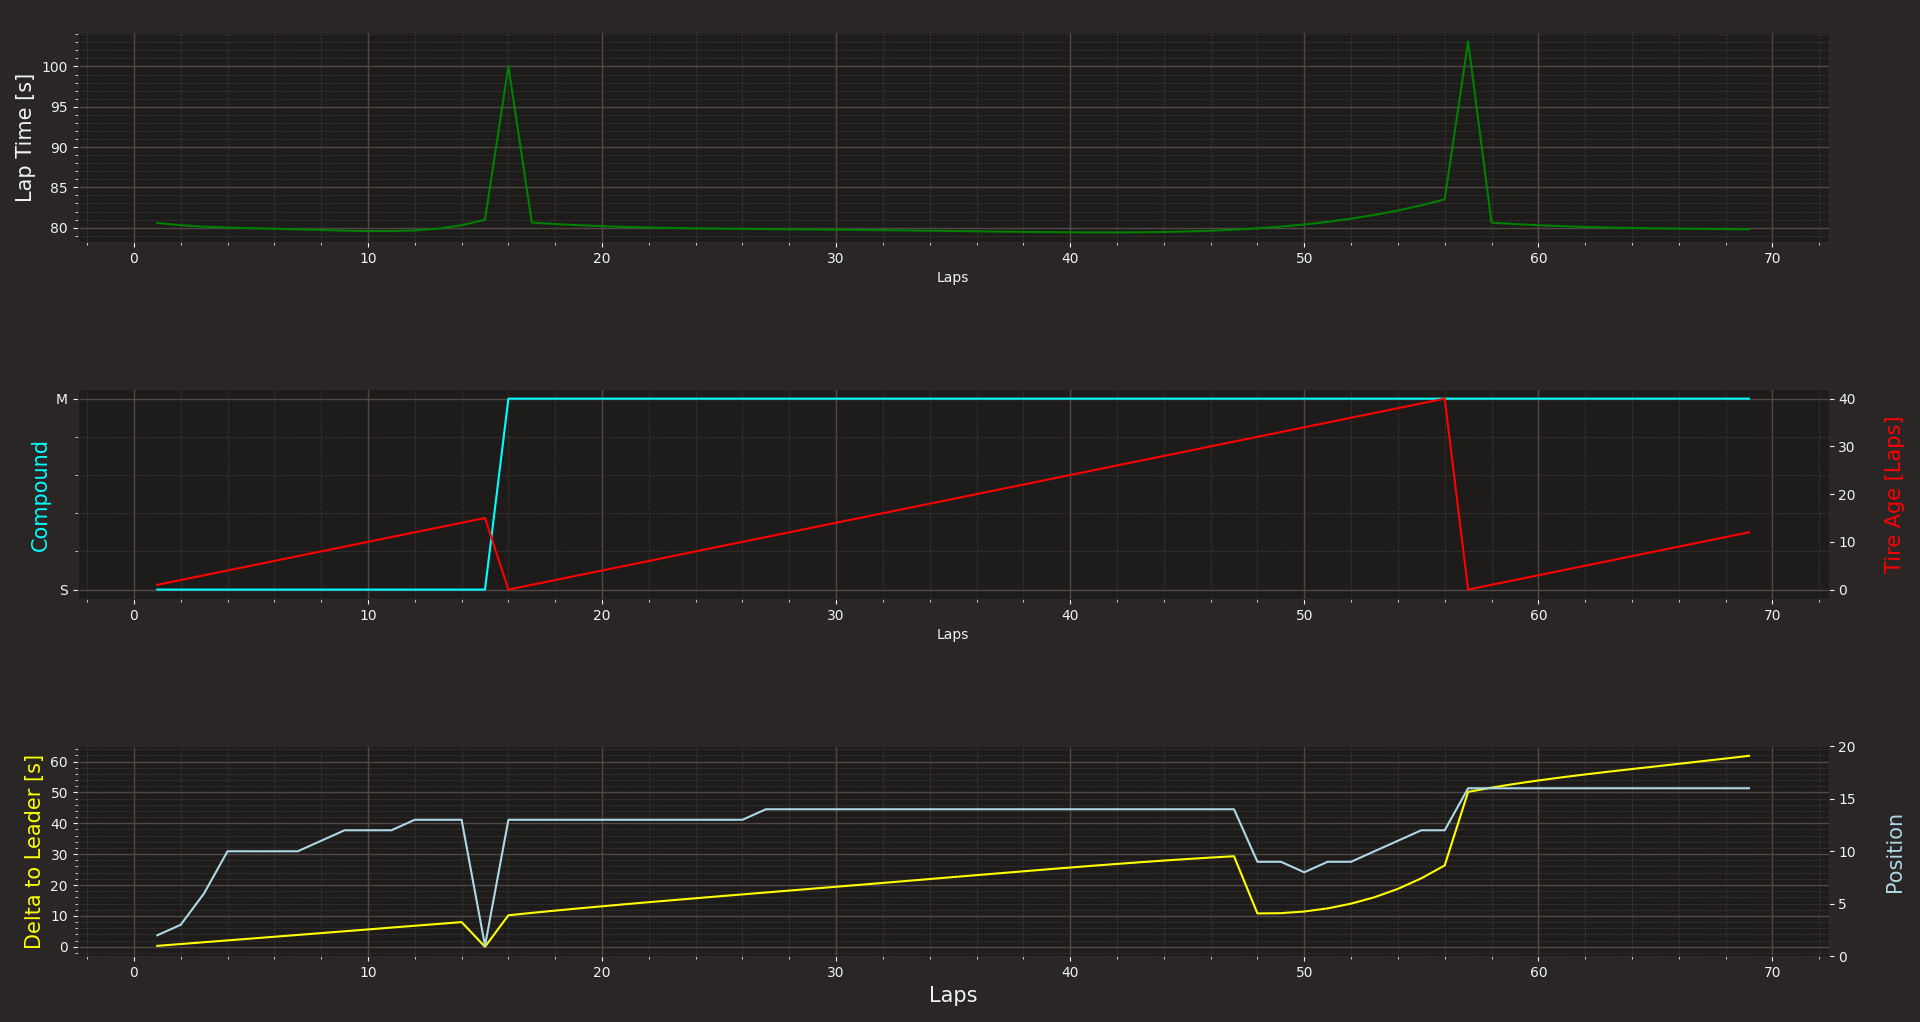
\includegraphics[scale=0.325]{Studienarbeit_F1/images/eval_worst_pole_new_got_16.png}
    \caption{Beispielhaftes Verhalten Szenario 2 - Start von Pole - Platz 15 im Ziel}
    \label{fig:example_scenario_two}
\end{figure}
Ebenfalls wird in diesem Szenario ein einzelnes Rennen beispielhaft in Abbildung \ref{fig:example_scenario_two} betrachtet. In diesem Fall ist besonders schön der Einfluss der Leistungsparameter auf die Rundenzeit durch die Individual-Modelle zu sehen. So verliert unsere KI kontinuierlich pro Runde an Zeit auf den Führenden (zu sehen im gelben Graph) trotz einer ähnlichen Strategie. Die Individual-Modelle funktionieren ebenso wie erwartet und erlauben eine reelle Abbildung der Leistung auf die Rennzeit als Ganzes. Dadurch kann unsere KI im schlechtesten Wagen die Führung nicht halten und landet auf Platz 15. Hierbei ist ebenfalls schön zu beobachten, dass die vorderen Positionen sehr schnell innerhalb von 15 Runden verloren werden, danach aber der Verlust langwierig ist. Dies resultiert aus den Leistungsunterschieden innerhalb des Fahrer-Feldes. Dabei befindet sich die KI zunächst in direktem Positionskampf mit den leistungsstärksten Konkurrierenden, welche entsprechend einfach die KI überholen können. Im späteren Rennverlauf befindet sich die KI im Umfeld schwächerer Gegner, welche nicht mehr in diesem Maße leistungsstärker sind und es folglich schwerer haben, dass leistungsschwächste Fahrzeug zu überholen. Dies bedeutet Überholen ist möglich, aber erst bei entsprechendem Tempo einfach. Ansonsten bleibt es eine Herausforderung, so wie es die reellen Verhältnisse vorgeben.


\subsubsection{Szenario 3: Leistungsstärkstes Auto ab letzter Start-Position}

Um eine tiefgreifendere Aussage über die Wechselwirkungsmodelle treffen zu können, muss entsprechend untersucht werden, ob das Überholen mit dem notwendigem Tempo zu leicht beziehungsweise zu schwer ist. Entsprechend wird hierbei ein Szenario gewählt, welches stark das Überholen fördert und provoziert, in dem die KI im performantesten Fahrzeug von der letzten Start-Position starten muss.\\
Hierbei wird kein Rennsieg erwartet, da dies in Anbetracht des restlichen Fahrerfeldes unrealistisch ist. Dennoch sollte ein klarer Fortschritt durch das Feld ersichtlich sein und die KI somit die Top 10 erreichen.
\\
\begin{figure}
    \centering
    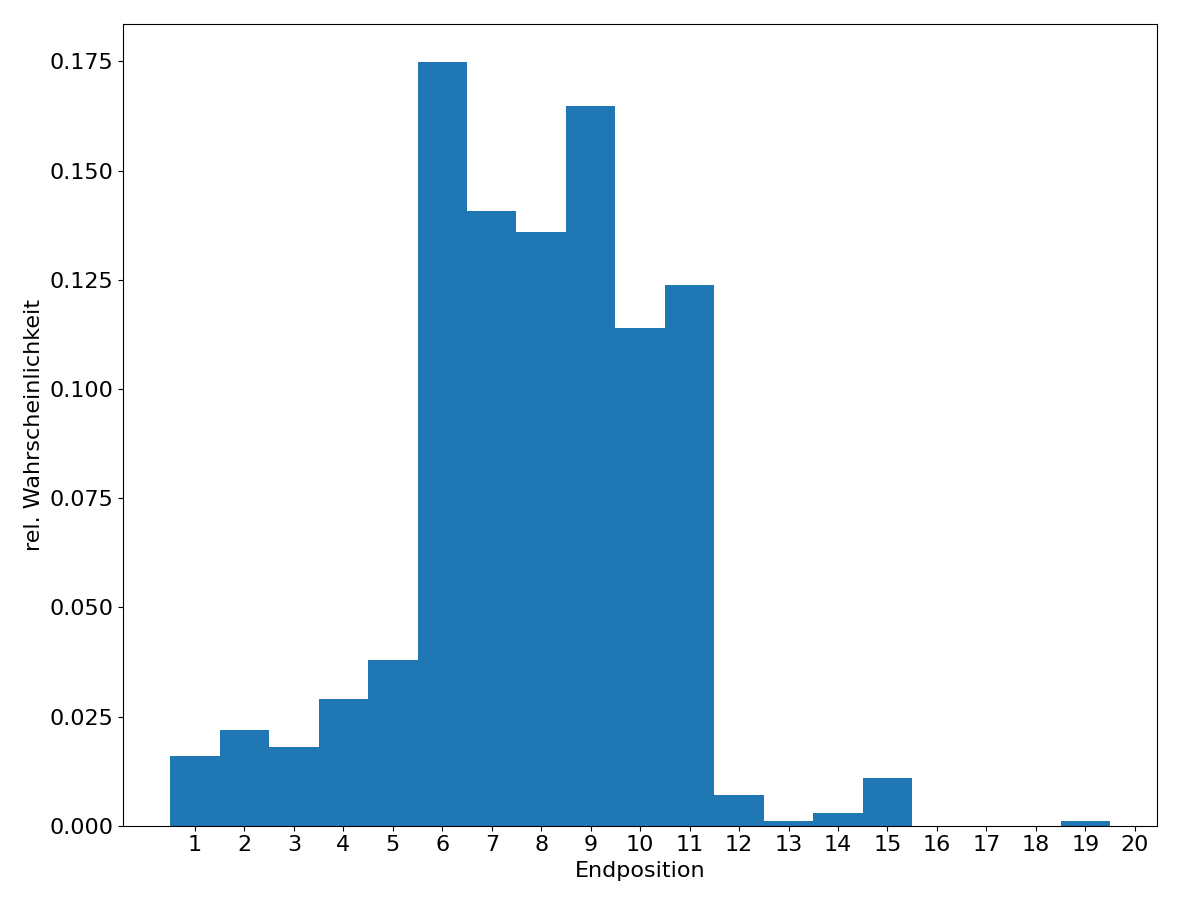
\includegraphics[scale=0.5]{Studienarbeit_F1/images/hist_best_car_from_back.png}
    \caption{Szenario 3: Anteile der Platzierungen bei 1000 Renndurchläufen}
    \label{fig:hist_best_car_from_back}
\end{figure}
\\
Im Zuge der längerfristigen Betrachtung der Resultate in Abbildung \ref{fig:hist_best_car_from_back} bestätigt sich die zuvor aufgestellte Vermutung an die Performance der KI. Es ist zu erkennen, dass die KI klare Erfolge innerhalb des Feldes erzielt und Plätze gut machen kann. Dies zeigt sich an dem sehr geringen Anteil an hinteren Positionen [12;20], die während der 1000 Renndurchläufe erzielt wurden.\\
Zeitgleich ist der Anteil an Podiumspositionen ebenfalls relativ gering, da in diesem Konkurrenzfeld gegen stärkere Gegner angetreten werden muss und ein Überholen mit weiterem Vorankommen deutlich erschwert wird.\\
Mit bei weitem größten Anteil hat die KI auf Basis dieser Leistungsparameter einen Rennabschluss in der Mitte des Feldes [6;11] erreicht. Damit kann die KI-Strategie in diesem Anwendungsszenario als stabil betrachtet werden.
\\
\begin{figure}
    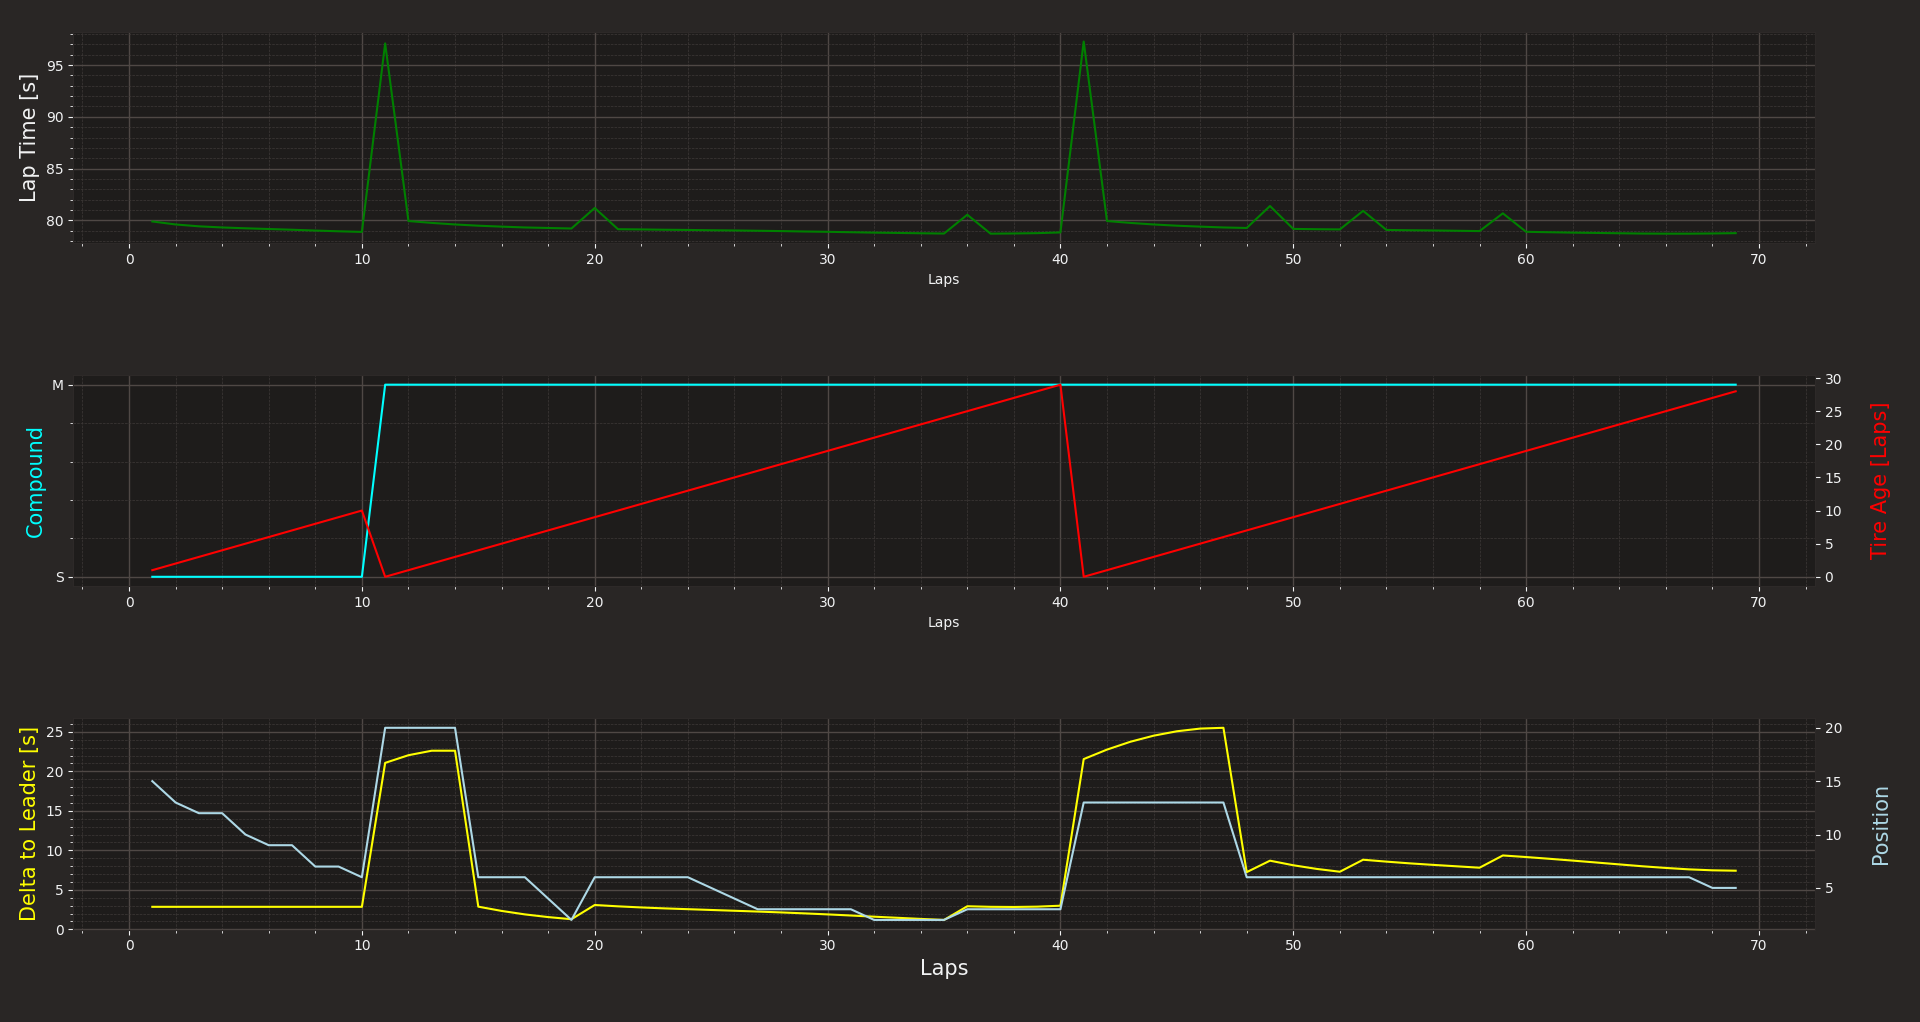
\includegraphics[scale=0.325]{Studienarbeit_F1/images/eval_best_from_last_new_got_5.png}
    \caption{Beispielhaftes Verhalten Szenario 3 - Start vom letzten Platz - Platz 5 im Ziel}
    \label{fig:example_scenario_three}
\end{figure}
\\
In der beispielhaften Untersuchung eines einzelnen Rennens in Abbildung \ref{fig:example_scenario_three} bestätigt sich die optimale Strategie mit einem initialem Stint auf Soft und zwei Stints auf Mediums, welche die KI wählt.\\
Aus Simulator Sicht sind an dieser Stelle die Ausreißer in der Rundenzeit interessant, welche neben den normalen Boxenstopps zu sehen sind. Diese zeigen deutlich, dass das Fahrzeug in diesen Runden an einem Überholmanöver scheiterte und so durch das restliche Fahrerfeld aufgehalten wurde. Dies bestätigt wiederum die Funktionsweise und Wirkung der Wechselwirkungsmodelle des Simulators.


\subsubsection{Szenario 4: Leistungsschwächstes Auto ab letzter Start-Position}

Um zusätzlich das Verhalten der KI vollständig zu verifizieren, wird in diesem Szenario der umgekehrte Fall zum Verhalten in \ref{sec:best_car_pole} untersucht. Entsprechend wird die schlechteste Ausgangslage für ein Formel 1 Fahrzeug angenommen mit schlechtestem Auto und der hintersten Start-Position. Hierbei liegt die Erwartung, dass die KI es potentiell schafft, einzelne Plätze gut zu machen durch die optimierte Strategie. Ein Erreichen der Top 10 ist aber allein durch die Modelle des Simulators höchst unwahrscheinlich.
\\
\begin{figure}[H]
    \centering
    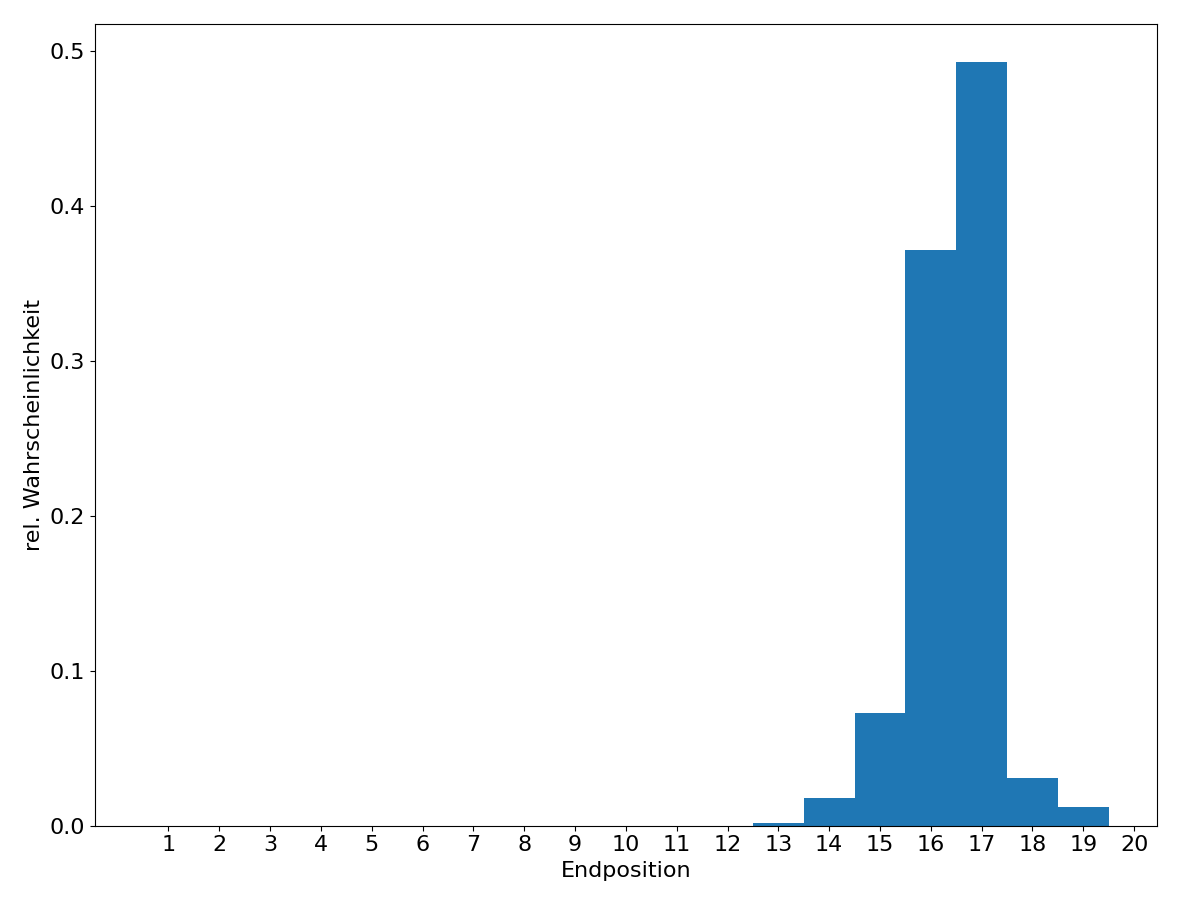
\includegraphics[scale=0.5]{Studienarbeit_F1/images/hist_worst_car_from_back.png}
    \caption{Szenario 4: Anteile der Platzierungen bei 1000 Renndurchläufen}
    \label{fig:hist_worst_car_from_back}
\end{figure}
Auch in diesem Szenario bestätigt sich das prognostizierte Verhalten, wie dem Histogramm \ref{fig:hist_worst_car_from_back} zu entnehmen ist. Aufgrund des leistungsstärkeren Konkurrenzfeldes ist es der KI nicht möglich, vordere Platzierungen zu erreichen, sondern befindet sich im Positionskampf mit schwächeren Gegnern im hinteren Teil des Feldes. Hier zeigt das Histogramm, dass es gelingt, einzelne Platzierungen gut zu machen und im Mittel Platzierungen um den 16 und 17 Rang zu erreichen. Dieses Ergebnis bestätigt den Vorteil der KI hinsichtlich der Rennstrategie, da es ihr gelingt, trotz eines leistungsschwachen Autos vereinzelte Plätze gutzumachen.
\\
\begin{figure}[H]
    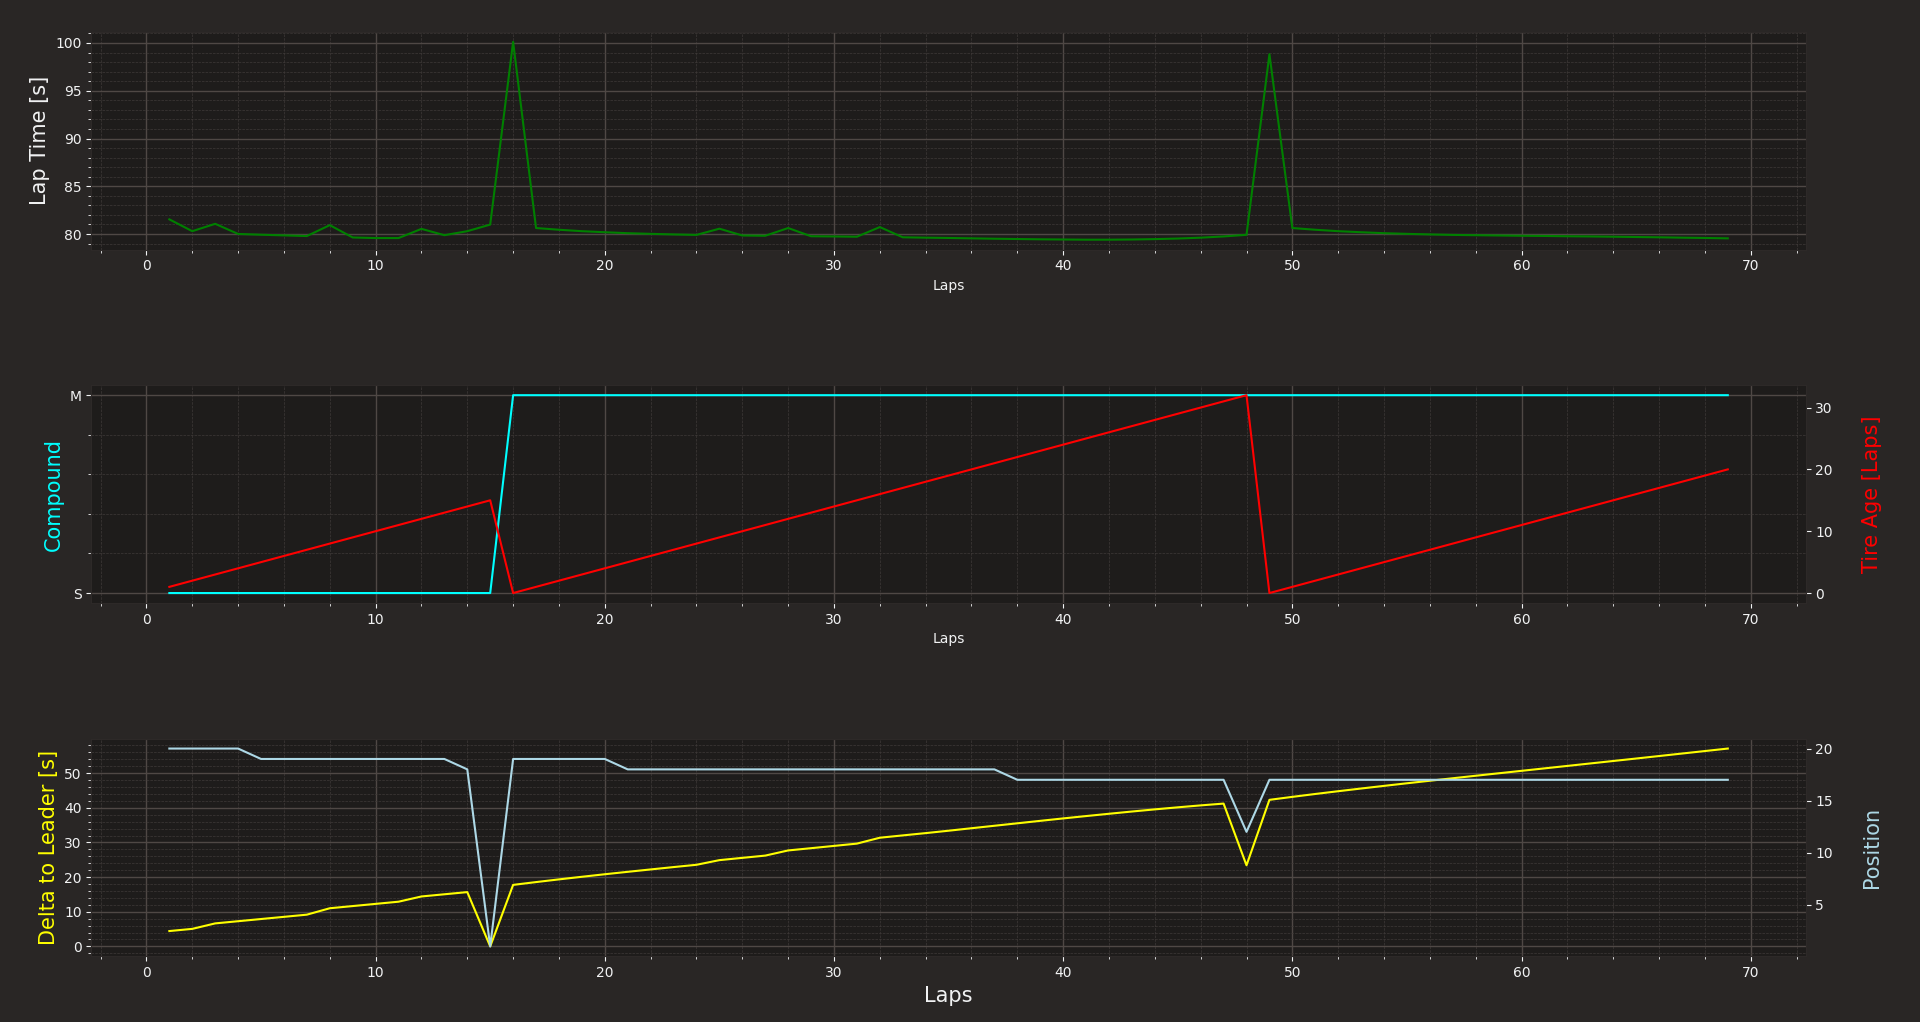
\includegraphics[scale=0.325]{Studienarbeit_F1/images/eval_worst_last_got_17.png}
    \caption{Beispielhaftes Verhalten Szenario 4 - Start vom letzten Platz - Platz 17 im Ziel}
    \label{fig:example_scenario_four}
\end{figure}
Auch in diesem Beispiel (siehe Abbildung \ref{fig:example_scenario_four}) sind die Einflüsse der anderen Fahrer im Feld deutlich in den Rundenzeit zu sehen. Dennoch schafft die KI mit besserer Strategie auch mit dem schlechtesten Fahrzeug einzelne Positionen gut zu machen und schafft somit den Sprung von Platz 20 auf Platz 17 im Ziel.\\\\
Im Allgemeinen ist über alle Szenarien hinweg auffallend, dass die KI identische Strategien wählt. Dieser Umstand wird im folgenden Kapitel \ref{sec:discussion} näher erläutert.



